
\section{Algoritmi}
\label{cap:algorithms}

\subsection{TSP 2-approssimato basato sul Minimum Spanning Tree}

La versione vista a lezione di questo algoritmo prevede i seguenti step:

\begin{enumerate}
    \item Selezionare un vertice radice $root$ arbitrario;
    \item Ricavare l'MST del grafo in input a partire da $root$, utilizzando ad esempio l'algoritmo di Prim;
    \item Eseguire una visita pre-order dell'MST ricavato al passo precedente;
    \item Aggiungere la radice $root$ pre-order alla fine della lista ritornata dalla visita pre-order.
    \item Calcolare il peso totale del circuito ricavato nei 2 passi precedenti e restituire il risultato.
\end{enumerate}

\noindent Il listato \ref{listing:tsp2approx} contiene la nostra implementazione dell'algoritmo, step per step.\\

\begin{listing}[!ht]
\begin{minted}{c++}
    // Step 1
    random_generator::IntegerRandomGenerator random(0, distance_matrix.size() - 1);
    const size_t root = random();

    // Step 2
    std::vector<Edge> mst(mst::prim_binary_heap_mst(distance_matrix, root));

    // Step 3, 4
    DFS dfs(std::move(mst));
    const auto circuit = dfs.preorder_traversal_rec();
    
    // Funzione lambda che calcola la distanza tra due vertici
    const auto get_distance = [&distance_matrix](const size_t x, const size_t y) {
        return distance_matrix.at(x, y);
    };
    
    // Step 5
    return utils::sum_weights_in_circuit(circuit.cbegin(), circuit.cend(), get_distance);
\end{minted}
\caption{Implementazione di TSP 2-approssimato. I commenti del file originale sono stati omessi per una maggiore compattezza.}
\label{listing:tsp2approx}
\end{listing}

\noindent L'algoritmo TSP 2-approssimato è stato implementato a partire dallo pseudo codice visto in classe. \\

\subsubsection{Osservazioni}

\begin{itemize}
    \item Abbiamo usato l'algoritmo di Prim perché è più adatto rispetto a Kruskal quando il grafo è rappresentato come matrice di adiacenza. Kruskal infatti richiede di estrarre la lista di lati ordinata in modo ascendente rispetto al peso all'inizio dell'algoritmo, mentre Prim richiede di estrarre solo la lista dei vertici. Ricordiamo che in un grafo completo vale l'equivalenza \complexityCompleteGraph{}.
    
    \item La coda di priorità usata dall'algoritmo di Prim è stata implementata con una Min Heap binaria.
\end{itemize}

\subsection{Held e Karp}

Riportiamo lo pseudocodice dell'algortimo di Held e Karp visto in classe. In particolare la funzione ricorsiva HeldKarp(v, S) si occupa di:

\begin{enumerate}
    \item Caso base: verificare se l'insieme S contenga un solo nodo, e restituire la distanza tra il nodo $v$ e 0.
    \item Controlla se la distanza tra 0 e v, passando per tutti i nodi in S, è già stata calcolata, restituendo tale valore.
    \item Caso ricorsivo:
    \begin{enumerate}
        \item Inizializzare le variabili in maniera opportuna.
        \item Scansionare tutti i nodi in S, togliendo v da S, e calcolare ricorsivamente la distanza. Se la distanza trovata è inferiore a quelle precedentemente ricavate, sostituirla.
    \end{enumerate}
    \item Ritornare la distanza minima calcolata.
\end{enumerate}


\noindent Il listato \ref{listing:held-karp} contiene la nostra implementazione dell'algoritmo, step per step.

\begin{listing}[!ht]
\begin{minted}{c++}
// HeldKarp.h

int held_karp_tsp_rec_bits_helper(timeout::timeout_signal& signal,
                                  DistanceMatrix<int>& distance_matrix,
                                  held_karp_dp_bits_t& C,
                                  utils::ull bits, size_t v = 0) {
    
    // Step 1
    if (utils::is_singleton(bits, v)) {
        return distance_matrix.at(v, 0);
    }

    // Step 2 
    if (C.count({bits, v})) {
        return C[{bits, v}];
    }
    
    // Step 3a
    int min_dist = std::numeric_limits<int>::max();
    const utils::ull difference = utils::reset_bit(bits, v);
    const size_t n = distance_matrix.size();

    // Step 3b
    utils::for_each(difference, n, [&](const size_t bit) {
        int dist = held_karp_tsp_rec_bits_helper(signal, distance_matrix, C,
                                                 difference, bit);
        int tmp_dist = dist + distance_matrix.at(v, bit);

        if (tmp_dist < min_dist) {
            min_dist = tmp_dist;
        }

        // Timeout scaduto: ritorna il miglior risultato ottenuto fino ad ora
        return !signal.is_expired();
    });
    
    // Step 4
    C[{bits, v}] = min_dist;
    return min_dist;
}

\end{minted}
\caption{Implementazione di Held e Karp con BitMasking. I commenti del file originale sono stati omessi per una maggiore compattezza.}
\label{listing:held-karp}
\end{listing}

\subsubsection{Osservazioni}

\begin{itemize}
    \item Abbiamo voluto riportare qui la versione con BitMasking a 64 bit, la versione con DynamicBitMasking è simile. Il controllo su quale delle due implementazioni usare è fatto prima di lanciare la funzione di ricorsione appropriata.\\
\end{itemize}

\newpage

\subsection{Farthest Insertion}

Farthest Insertion è un'euristica costruttiva per TSP che consente di
approssimare la soluzione ad un fattore $\log(n)$, ulteriormente
abbassabile fino ad un fattore $2$. La complessità asintotica di
quest'euristica è $\bigO(n)$.

\subsubsection{Idea}

L'euristica è molto semplice e utilizza un'insieme di regole per
scegliere il punto di partenza, il vertice da inserire ad ogni
iterazione e la posizione in cui inserire il nuovo vertice. In
particolare:

\begin{enumerate}
    \item Inizializzazione: considera il circuito parziale composto
      dal solo vertice $0$. Trova un vertice $j$ che minimizza $w(0,
      j)$ e costruisci il circuito parziale $(0, j,0)$;
    \item Selezione: trova un vertice $k$ non presente nel circuito
      parziale $C$ che massimizza $\delta(k,C)$;
    \label{pseudo:farthest-insertion-selection}
    \item Inserimento: trova l’arco ${i, j}$ del circuito parziale che
      minimizza il valore $w(i, k) + w(k, j) - w(i, j)$ e inserisci
      $k$ tra $i$ e $j$;
    \item ripeti da \ref{pseudo:farthest-insertion-selection} finché
      non hai inserito tutti i vertici nel circuito.
\end{enumerate}

\subsubsection{Algoritmo}

\noindent Il listato \ref{listing:farthest-insertion} contiene la
nostra implementazione dell'algoritmo.

\begin{listing}[!ht]
\begin{minted}{c++}
// farthest_insertion_tsp.h

const size_t size = distance_matrix.size();

// Funzione lambda per il calcolo della distanza tra due vertici-
const auto get_distance = [&distance_matrix](const size_t x, const size_t y) {
    return distance_matrix.at(x, y);
};

// Insieme degli nodi ancora non visitati.
std::unordered_set<size_t> not_visited = utils::generate_range_set(size);

// Comparatore per massimizzare d(k, circuit)
using max_comparator = std::less<>;

// Inizializzazone.
const size_t first_node = rand_int();
const size_t second_node = distance_matrix.get_closest_node(first_node);

std::vector<size_t> circuit{first_node, second_node};
circuit.reserve(size);

not_visited.erase(first_node);
not_visited.erase(second_node);

// Selezione del nodo k che massimizza d(k, circuit).
const size_t k = utils::select_new_k<max_comparator>(
    not_visited, circuit, get_distance);

// Inserimento del k trovato tra due nodi i e j in modo tale da
// minimizzare la distanza totale del cammino.
circuit.emplace_back(k);
not_visited.erase(k);

// Ripetere selezione e inserimento finché tutti i nodi non sono stati inseriti.
while (!not_visited.empty()) {
    size_t new_k = utils::select_new_k<max_comparator>(
        not_visited, circuit, get_distance);
    not_visited.erase(new_k);

    utils::perform_best_circuit_insertion(new_k, circuit, get_distance);
}

// Restituire la somma dei pesi del circuito trovato.
return utils::sum_weights_in_circuit(circuit.cbegin(), circuit.cend(), 
                                     get_distance);
\end{minted}
\caption{Implementazione di Farthest Insertion. I commenti del file originale sono stati omessi per una maggiore compattezza.}
\label{listing:farthest-insertion}
\end{listing}

\subsubsection{Osservazioni}

\begin{itemize}
    \item All'algoritmo viene passata la matrice delle adiacenze e un
      random generator per la selezione del primo nodo durante
      l'inizializzazione. (Ulteriori dettagli in
      \ref{sec:farthest-insertion-rounds}).

    \item L'insieme \mintinline{c++}{not_visited} è utilizzato per
      tenere traccia degli elementi presenti nel circuito Hamiltoniano
      parziale: ogni volta che un vertice è inserito nel circuito,
      viene rimosso dall'insieme.

    \item L'operazione $\min w(i, j)$ è rappresentata dalla funzione
    \begin{center}
        \mintinline{c++}{get_closest_node(node)}
    \end{center}
    invocabile sulla matrice di adiacenza, utilizzata nella fase di
    inizializzazione.

    \item L'operazione di massimizzazione di $\delta(k, C)$ è
      rappresentata dalla funzione
    \begin{center}
        \mintinline{c++}{utils::select_new_k<max_comparator>(not_visited,
          circuit, get_distance);}
    \end{center}
    che sceglie il vertice $k$ che massimizza (o minimizza, in base al
    comparatore fornito) la distanza tra $k$ ed il circuito $C$. Per
    farlo in input riceve l'insieme dei nodi non ancora in $C$ da cui
    scegliere $k$, $C$ e la funzione di distanza.

    \item L'inserimento del vertice selezionato è effettuato in
    \begin{center}
        \mintinline{c++}{utils::perform_best_circuit_insertion(new_k,
          circuit, get_distance);}
    \end{center}
    che sceglie la posizione di inserimento che minimizza la distanza
    massima del circuito.
\end{itemize}


\subsubsection{Rounds}
\label{sec:farthest-insertion-rounds}

\noindent L'euristica prevede un'inizializzazione statica del
problema, scegliendo sempre il primo nodo come il vertice 0. In
realtà, scegliendo nodi diversi come sorgente le soluzioni ritornate
dall'algoritmo potrebbero differire, e molteplici esecuzioni
dell'algoritmo da diverse sorgenti potrebbero produrre soluzioni più
accurate rispetto ad una singola esecuzione.\\

\noindent Abbiamo deciso di sfruttare questo fatto implementando la
possibilità di eseguire l'algoritmo in parallelo su diversi core.\\

\noindent All'algoritmo è infatti passato un
\mintinline{c++}{RandomGenerator} che consente di generare un numero
casuale, rappresentante la sorgente del ciclo Hamiltoniano da
costruire. In realtà, il random generator è fornito in diverse
implementazioni:
\begin{itemize}
    \item \mintinline{c++}{RealRandomGenerator}, generatore per numeri
      casuali di tipo reale;
    \item \mintinline{c++}{IntegerRandomGenerator}, generatore per
      numeri casuali di tipo intero;
    \item \mintinline{c++}{FixedGenerator}, generatore del numero
      specificato al momento della creazione del generator.
\end{itemize}
L'inizializzazione di Farthest Insertion può quindi differire in base
al generator fornito in input: se il generator è un
\mintinline{c++}{FixedGenerator} allora la sorgente scelta è fissata,
altrimenti la sorgente è scelta in modo casuale.\\

\noindent Nel nostro caso abbiamo eseguito l'algoritmo prima con
sorgente fissata a $0$ e poi con sorgente random e fissando il numero
di istanze parallele a $4$: i risultati sono stati soddisfacenti,
infatti come si può notare dal grafico
\ref{fig:farthest-insertion-1-4-rounds-accuracy-error}, l'esecuzione
multipla dell'algoritmo tende a restituire soluzioni più corrette.\\

\begin{figure}[H]
    \centering

    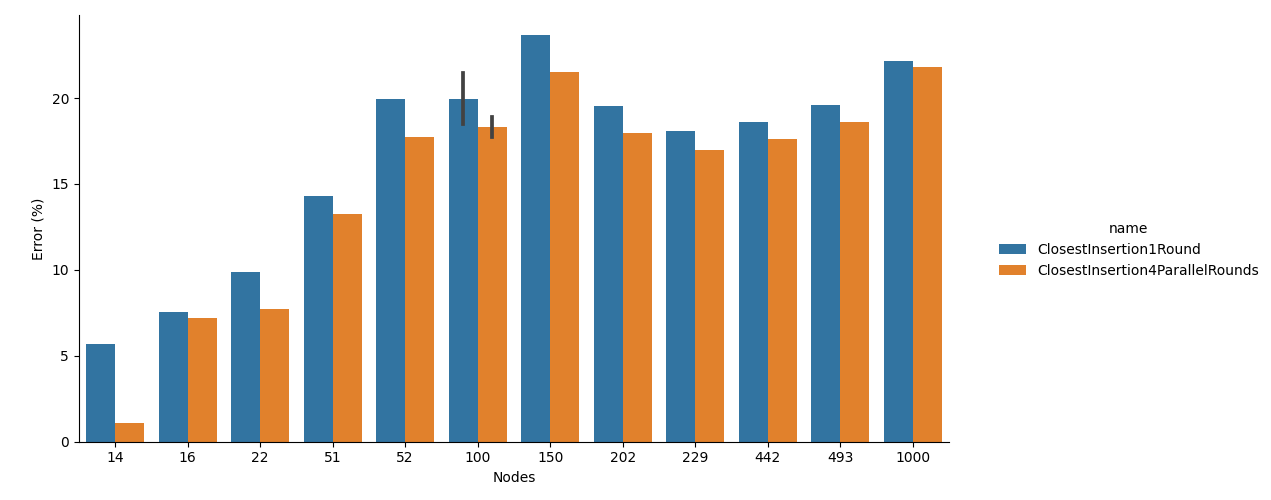
\includegraphics[width=0.9\textwidth]{./images/ClosestInsertion1Round_vs_ClosestInsertion4ParallelRounds__approximation_error_.png}

    \caption{ClosestInsertion accuracy error scaling by nodes}
    \label{fig:farthest-insertion-1-4-rounds-accuracy-error}
\end{figure}
